\documentclass[12pt,onecolumn%,twoside
]{scrartcl}
\usepackage[utf8]{inputenc}
\usepackage[english,ngerman]{babel}
\usepackage[pdfusetitle]{hyperref}
\usepackage{graphicx}
\usepackage{calc}
\usepackage{caption}
\usepackage{fancyhdr,multicol,multirow,bigdelim,paralist,graphicx,array,enumitem}
\usepackage{amsmath, mathtools}
\usepackage{float}
\usepackage{color}
\usepackage[dvipsnames]{xcolor}
\renewcommand{\sectionmark}[1]{\markboth{#1}{}}
\addto\captionsngerman{\renewcommand{\figurename}{Figure}}
\addto\captionsngerman{\renewcommand{\contentsname}{Index}}
\KOMAoptions{parskip=half+,paper=a4,twocolumn=false,DIV=12}
\fancypagestyle{eca-style}{
\fancyhf{}
\fancyhead[L]{ECA}
\fancyhead[R]{\leftmark}
\fancyfoot[C]{\thepage}
\renewcommand{\headrulewidth}{0.4pt}
\renewcommand{\footrulewidth}{0.4pt}}
\fancypagestyle{index-style}{
\fancyhf{}
\fancyhead[L]{ECA}
\fancyhead[R]{Index}
\fancyfoot[C]{\thepage}
\captionsetup{width=0.5\textwidth}
\renewcommand{\headrulewidth}{0.4pt}
\renewcommand{\footrulewidth}{0.4pt}}
\setdescription{itemsep=0pt}
\makeatletter
\newenvironment{minipagespace}{
\begin{minipage}
}{
\end{minipage}
\vspace{10pt}
}
\makeatother
\setcounter{tocdepth}{3}
\title{Enumerative Combinatoric Algorithms (716.035)}
\date{2016}

\DeclarePairedDelimiter\ceil{\lceil}{\rceil}
\DeclarePairedDelimiter\floor{\lfloor}{\rfloor}

\newcommand{\img}[3]{
\begin{figure}[H]
	\centering
	\includegraphics[#2]{img/#1}
	\captionsetup{width=0.8\textwidth, justification=centering}
	\caption{#3}
\end{figure}
}

\newcommand{\imgnc}[2]{
\begin{figure}[H]
	\centering
	\includegraphics[#2]{img/#1}
	\captionsetup{width=0.8\textwidth, justification=centering}
\end{figure}
}

\newcommand{\fig}[2]{
\begin{figure}[H]
	\centering
	#1
	\captionsetup{width=0.8\textwidth, justification=centering}
	\caption{#2}
\end{figure}
}

\newcommand{\eq}[1]{
\begin{equation*}
\begin{aligned}
#1
\end{aligned}
\end{equation*}
}

\newcommand{\mat}[1]{
\begin{pmatrix}
#1
\end{pmatrix}
}

\newcommand{\newsection}[1]{
\cleardoublepage
\section{#1}
}

\newcommand{\st}[4]{
\boxed{\text{#1}}\boxed{\text{#2}}\boxed{\text{#3}}\boxed{\text{#4}}
}

\begin{document}

\begin{titlepage}
\maketitle
\newpage
\pagestyle{index-style}
\tableofcontents{}
\newpage
\end{titlepage}

%%%%%%%%%%%%%%%%%%%%%%%%%%%%%%%%%%%%%%%%%%%%%%%%%%%%%%%%%%%%%%%%%%%%%%%%%%%%%%%%%%%%%%%%%%%%

\pagestyle{eca-style}

\newsection{Enumerating vs. Counting}

\subsection{Permutation of Letters}

{\bf Example:} How many words can we make out of the letters A B C using each letter once?

\begin{center}
\begin{inparaitem}
	\item ABC \qquad
	\item BAC \qquad
	\item CAB
\end{inparaitem}

\begin{inparaitem}
	\item ACB \qquad
	\item BCA \qquad
	\item CBA
\end{inparaitem}
\end{center}

When we list all objects as above we call it {\bf enumeration}, whereas {\bf counting} is only concerned with the total number of objects. If we consider the example above, how many words would be possible for A B C D?

It's best to find a formula, as using it is a very efficient way to count objects. For $n = 4$ letters we end up with $24$ permutations.

The formula for the amount of different words with $n$ letters is $n!$

\subsection{Points in Convex Position}

How many crossing-free spanning paths exist for $n$ points on convex position?

\img{crossing_free_spanning_path}
    {scale=1.5, trim=220 550 430 125}
    {An example illustrating one possibility of a spanning path for $n=9$ points}

For $n=1$ points the definition of the spanning path is unclear, in some cases it is considered as path with the size $1$ and in others with size $0$.

Let's look at some examples for $n > 1$ and try to determine a suitable formula. 

\img{crossing_free_spanning_path_enumeration}
    {scale=1, trim=270 340 200 125}
    {Enumeration of crossing free spanning paths up to $n=4$}

As we can see from this example, enumeration can become a tedious and error prone task very fast. Can you list all paths for $n=5$?

It is better to abstract the problem and find an inductive solution. When constructing the path we start with a point, and from it we only see two immediate choices. After one of those points is added, we have two choices again. This goes on for a while until $n-2$.

\eq{\underbrace{2 \cdot 2 \cdot 2 \cdots 2 \cdot 2}_{n-2 \text{ times}} = 2^{n-2}}

Now in order to construct all paths we need to start at all possible points, when we do that however a double count occurs.

\eq{n \cdot 2^{n-2} \Rightarrow \frac{n \cdot 2^{n-2}}{2} \Rightarrow n \cdot 2^{n-3} \text{ for } n \ge 2 }

We can use this formula to find the number of crossing-free spanning paths for $n=5$, which gives us $5 \cdot 2^2 = 20$ paths.

\img{crossing_free_spanning_path_n_5}
    {scale=1, trim=200 425 200 125}
    {Another method of enumeration, do not explicitly list similar objects}
    
\newsection{Polyominos}

\img{polyominos}
	{scale=1, trim=225 555 200 125}
	{A polyomino of size $n$ consists of $n$ unit squares connected via edges, aligned on a grid}
	
\img{polyominos_holes}
	{scale=1, trim=235 505 360 140}
	{A polyomino with a hole inside. Polyominos without holes are a special case and they are called animals.}	
	
How many n-polyominos do exist? We have to define how to count them, that means defining the parameters that decide when two polyominos are regarded as one and the same. Polyominos can be compared using three operations:
\begin{enumerate}
	\item {\bf Translation}: Move one polyomino on top of another, if they overlap, they are the same.
	\item {\bf Rotation}: Additionally rotate one polyomino, if there is one rotation that makes them overlap, they are the same.
	\item {\bf Reflection}: Move in the 3$^{rd}$ dimension, mirroring the polyomino.
\end{enumerate}

With these operations polyominos can be classified into these two groups: 
\begin{itemize}
	\item {\bf Fixed polyominos}: Only translation is allowed.
	\item {\bf Free polyominos}: Translation, rotation and reflection is allowed.	
\end{itemize}

\fig{
\begin{tabular}{| r | c | c |}
  \hline
  n & \# fixed & \# free \\
  \hline	
  1 & 1 & 1 \\
  2 & 2 & 1 \\
  3 & 6 & 2 \\
  4 & 19 & 5 \\
  5 & 63 & 12 \\
  \vdots & \vdots & \vdots 
\end{tabular}}{How many n-polyominos do exist?}

What is the formula for generating \underline{all} n-polyominos? Look at a step from $n \to n+1$, we can add one unit square to all surfaces, in the absolute worst case (a straight polyomino) that means $2n+2$ possibilities. How can we best deal with duplicates?

{\bf Approach 1}: Generate all new polyominos, then compare them all. For size $n+1$, $k$ polyominos are generated. $\Rightarrow O((_2^k) \cdot n) = O(k^2 \cdot n)$ 

Problem: $k >> n$

{\bf Approach 2}: Fingerprinting. Build a vector of a polyomino that is given by the coordinates of the squares.

\img{polyominos_vector}
	{scale=1, trim=275 505 360 125}
	{Polynomios and their respective vector fingerprint.}
	
Compute all eight polyonimos (4x rotation \& 2x reflection) and take the lexicographical minimum of the vector form!

Time for the fingerprint: $O(n)$

$\Rightarrow$ Compute fingerprints of all generated polyominos: $O(k \cdot n)$

$\Rightarrow$ Sort all fingerprints: $O(k \cdot log(k) \cdot n)$, duplicates are neighboured in the sorting and removing takes $O(k \cdot n)$
$\Rightarrow$ the total runtime is $O(k \cdot log(k) \cdot n)$

No formula is known for the number of fixed/free polyominos.

\eq{\lim\limits_{n \rightarrow \infty}\frac{\# (n+1) \text{ polyominos}}{\# n \text{ polyominos}} = \text{some constant } c}

The number of polyominos goes to $\Theta(c^n)$ and we know that $4.00253 \le c \le 4.65$.

\newsection{Pigeonhole-Principle}

Also known as Dirichlet principle, or in German $"$Schuhfach Prinzip$"$.

If you have $n+1$ elements (pigeons) which you put into $n$ boxes (pigeonholes), then there is a box with at least two elements (two pigeons).

{\bf General form}: If you have $k$ elements which you put into n boxes, then there is a box with at least $\ceil*{\frac{k}{n}}$ and one with at most $\floor*{\frac{k}{n}}$ elements.

\subsection{Example 1: Socks}

You have $n$ black socks and $m$ white socks in a drawer. How many socks do you have to pick out in order to get a matching pair?

If you abstract the problem using the pigeonhole principle it leads to the following setup. In total there are $n+m$ elements that are distributed upon two boxes, one for white socks and one for black socks. If we pick a sock out of the drawer and put it into one of the two boxes, we have to repeat the process at least three times to have a box with two elements in them (a matching pair of socks).

For $n=2$ boxes there have to be $n+1=3$ elements, such that one of the boxes contains at least $\ceil*{\frac{3}{2}} = 2$ elements.

\subsection{Example 2: Numbers}

Let $S$ be a subset of $\{1,2,\cdots, 2n\}$ of cardinality $n+1$. Prove or give a counter example for: $S$ contains two numbers $a$ and $b$ such that
\begin{itemize}
\item $a+b = 2n + 1$
\item $a-b = n$
\end{itemize}

To solve this problem we have to think of appropriate labels for the boxes.

\begin{center}
\begin{tabular}{l  l}
  $\{1,2n\}$ & \rdelim\}{5}{1mm}[ $n$ boxes]\\
  $\{2,2n-2\}$ & \\
  $\{3,2n-3\}$ & \\
  $\qquad\vdots$ & \\
  $\{n,n+1\}$ &  
\end{tabular}
\end{center}

There is a subset of cardinality $n+1$, so taking a number and putting it into the box with its name on the label, there has to be at least one box with two elements, thus adding up to $2n+1$.

\newpage

Similarly, solve the second problem by using different labels
\begin{center}
\begin{tabular}{l  l}
  $\{1,n+1\}$ & \rdelim\}{5}{1mm}[ $n$ boxes]\\
  $\{2,n+2\}$ & \\
  $\{3,n+3\}$ & \\
  $\qquad\vdots$ & \\
  $\{n,\underbrace{n+n}_{2n}\}$ &  
\end{tabular}
\end{center}

\subsection{Example 3: Hairs}

Prove: In Austria there exist at least eight people with the same number of hairs on their head.

Facts:
\begin{itemize}
\item On average people have $150.000$ hairs
\item It is save to assume that the range is $0-1.000.000$
\item Population of Austria: $8.699.730$ (Jan 1$^{st}$ 2016)
\end{itemize}

Take the total range of hairs as boxes, leading to $1.000.001$ boxes. At least $\ceil*{\frac{8699730}{1000001}} \sim \ceil*{8,7} = 9$ people have the same number of hairs on their head in Austria.

\subsection{Example 4: Party}

At a party $n \ge 2$ people meet. Some shake hands with others and some don't. Show or provide a counter example:
\begin{itemize}
\item There are at least two people at this party shaking the same number of hands.
\end{itemize}

There are two cases to consider for the boxes.

\begin{enumerate}
\item No one shakes zero hands.

\begin{tabular}{l  l}
  \multicolumn{2}{c}{\# handshakes} \\
  $1$ & \rdelim\}{5}{1mm}[ $n-1$ boxes]\\
  $2$ & \\
  $3$ & \\
  $\vdots$ & \\
  $n-1$ &  
\end{tabular}
\item At least one person shakes zero hands

\begin{tabular}{l  l}
  \multicolumn{2}{c}{\# handshakes} \\
  $0$ & \rdelim\}{5}{1mm}[ $n-1$ boxes]\\
  $1$ & \\
  $2$ & \\
  $\vdots$ & \\
  $n-2$ &  
\end{tabular}
\end{enumerate}

In both cases we have $n-1$ boxes for $n$ elements, meaning there always has to be a box with at least two elements.

\subsection{Example 5: Numers II}

Let $q$ be an odd number and let $S$ be the set $\{1,3,7,15,31, \cdots , 2^i-1\}$, i.e. $S$ contains the elements $a_i = 2^i-1$ for all $i \ge 1$.

{\bf Claim}: For each odd number $q$ there exists an $a_i$ which is a multiple of $q$ ($q$ divides $a_i$ without rest)

\eq{a_i = c \cdot q + r_i \qquad r_i \text{ has to be zero}}

Boxes for the rest:

\begin{tabular}{l  l}
  $\{r_i = 0\}$ & \rdelim\}{5}{1mm}[ $q$ boxes]\\
  $\{r_i = 1\}$ & \\
  $\{r_i = 2\}$ & \\
  $\qquad \vdots$ & \\
  $\{r_i = q-2\}$ &  
\end{tabular}

We can ignore the case with at least one element in box $\{r_i = 0\}$, since it means we are done already. If we ignore that box, there have to be two boxes with the same rest.

\eq{
	 		& a_m = c^* \cdot q + r_m \\
	- \quad & \underline{a_m = c^{**} \cdot q + r_m} \\
	 		& a_m - a_n = c^{***} \cdot q \qquad m > n \\
	 		& a_m - a_n = 2^m-1-(2^n-1) = \\
	 		& 2^m-2^n = 2^n\underbrace{(2^{m-n}-1)}_{a_{m-n}}
}

$a_{m-n}$ must be a multiple of $q$.

\newsection{Inclusion-Exclusion}

{\bf Example}: How many numbers of the set $\{1 \dots 45\}$ are coprime (do not have a common divisor) with 45?

We can use the following equation to find a solution.
\eq{X = 45 - |\{ \text{numbers which have at least one common divisor with 45} \}|}

For that we need to take a look at the prime coefficients of $45$ which consist of $3 \cdot 3 \cdot 5$ and count the members of the set divisible by them.
\eq{
	X_i &= | \text{numbers of } \{1 \dots 45\} \text{ divisible by i} | \\
	X_3 &= \frac{45}{3} = 15 \\
	X_5 &= \frac{45}{15} = 9 \\
	X_{3 \cdot 5} = X_{15} &= \frac{45}{15} = 3
}

In the last line, we made preparations to ensure that no double count occurs. 
\eq{
	X &= 45 - X_3 - X_5 + X_{3 \cdot 5} = 45 - 15 - 9 + 3 = 24
}

{\bf Lemma}: For two sets $A,B$ we are interested in $|A \cup B|$
\eq{|A \cup B| = |A| + |B| - |A \cap B|}

{\bf Example 2}: How many numbers of the set $\{1 \dots 60\}$ are coprime with 60?
\eq{
	60 &= 2 \cdot 2 \cdot 3 \cdot 5 \\
	X &= 60 - \underbrace{X_2}_{30} - \underbrace{X_3}_{20} - \underbrace{X_5}_{12} + \underbrace{X_6}_{10} + \underbrace{X_{10}}_{6} + \underbrace{X_{15}}_{4} - \underbrace{X_{30}}_{2} \\
	X &= 16
}

{\bf Lemma}: For three sets $A,B,C$ we are interested in $|A \, \cup \, B \, \cup \, C|$
\eq{|A \cup B \cup C| = |A| + |B| + |C| - |A \cap B| - |A \cap C| - |B \cap C| + |A \cap B \cap C|}

%TODO insert full formula here

\subsection{Spanning trees in ladders}

\img{ladder_spoke}
    {scale=1, trim=200 420 450 120}
    {Depiction of a ladder as a connected, cycle-free spanning tree. A ladder of size $n$ 		has $n$ spokes.}
    
How many spanning trees does a ladder of size $n$ contain as subgraphs (with the same vertex set)?

\imgnc{ladder_subgraphs}{scale=1, trim=100 425 100 120, clip}

\imgnc{ladder_subgraphs}{scale=1, trim=100 275 100 370, clip}

\imgnc{ladder_subgraphs_n3}{scale=1, trim=100 400 100 125, clip}

For the total number of subgraphs with a ladder of size $n=3$ we can calculate \\ $3+8+4=15$ 

How many spanning trees does a ladder of size $n=4$ contain as subgraphs? How can we find a formula for this problem? We need to make some definitions!

\eq{
	X_A (n) \dots \# &\text{ of spanning trees in a ladder of size } n \\
	X_B (n) \dots \# &\text{ of spanning graphs which consist of \underline{2} components} \\
					 &\text{ and are cycle free for a ladder of size } n \text{ such that} \\
					 &\text{ the rightmost 2 vertices are in \underline{different}} \\
					 &\text{ components.}
}

We can then build the following table:

\begin{center}
\begin{tabular}{c | c | c}
  $n \rightarrow n+1$ & start with $X_A (n)$ & start with $X_B (n)$ \\
  \hline
  \raisebox{3.7\height}{$X_A (n+1)$} &  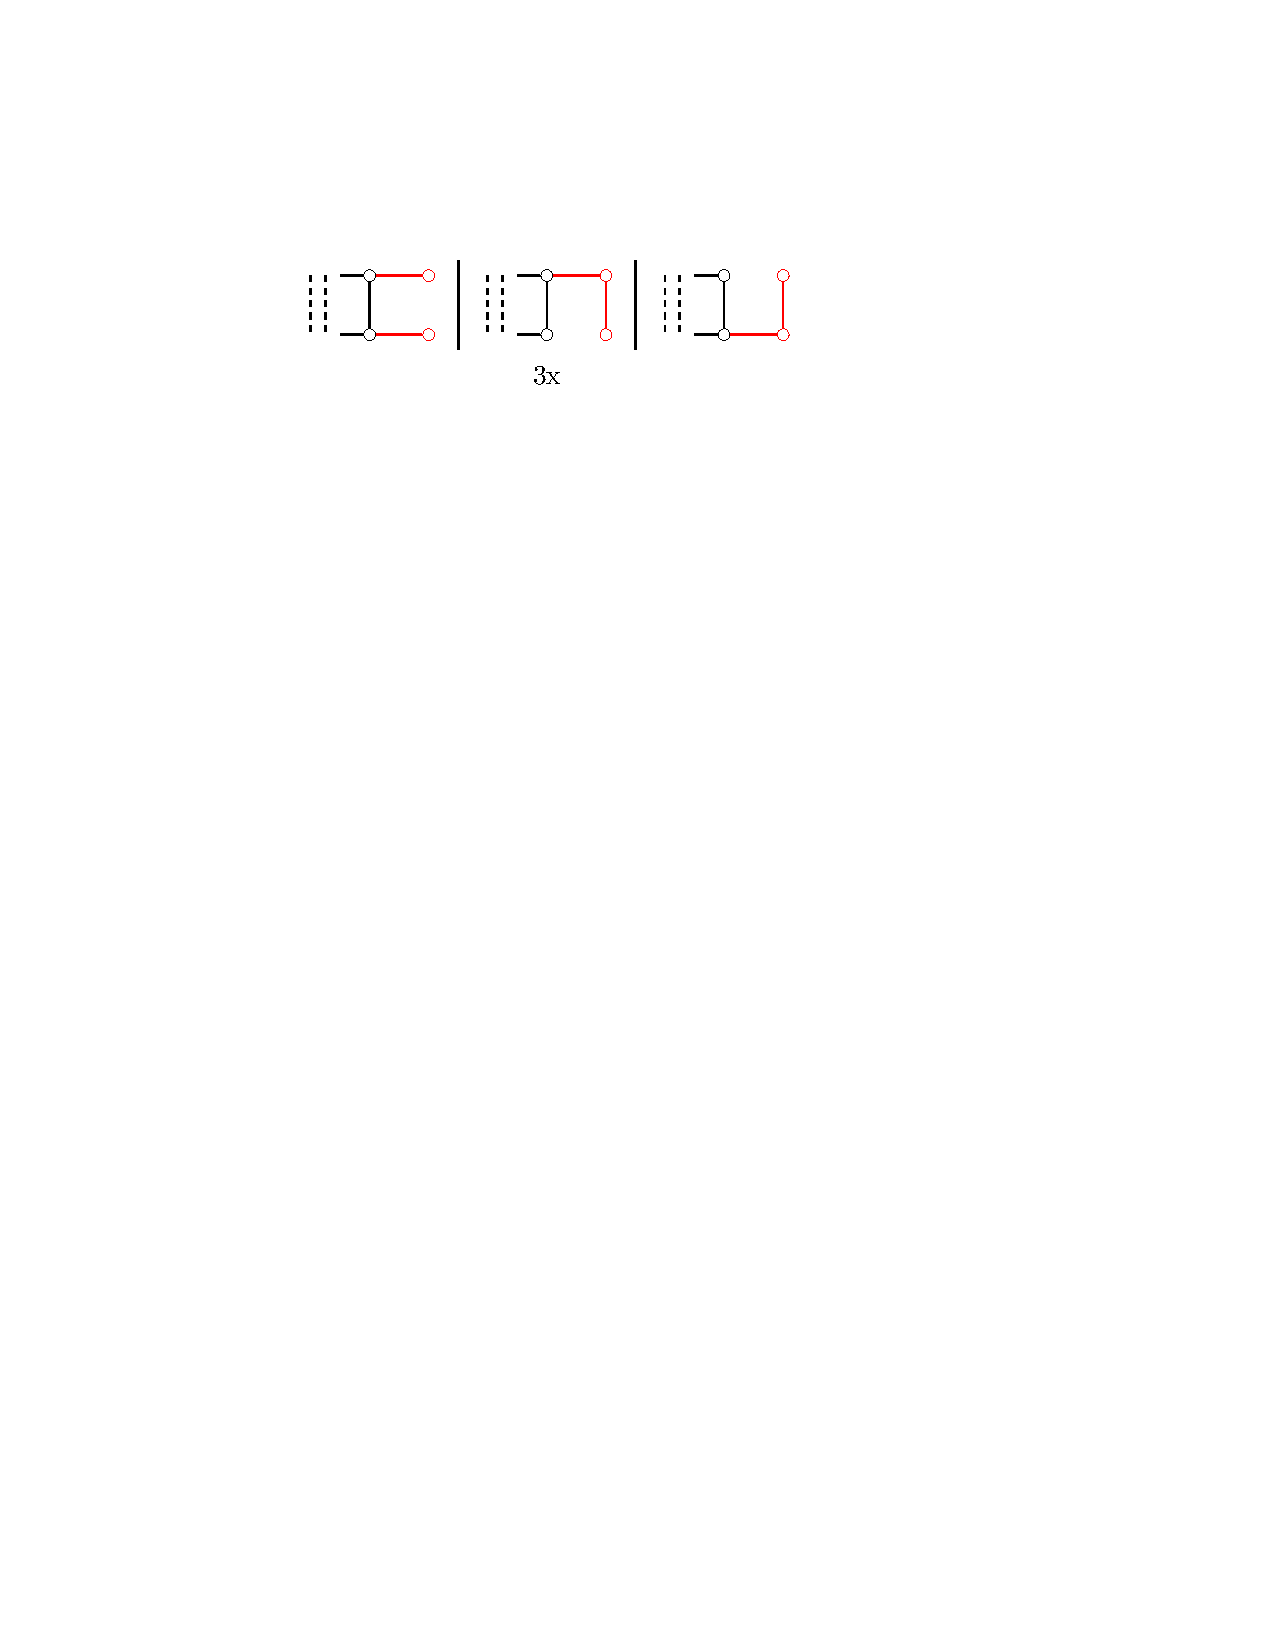
\includegraphics[trim=130 600 220 110,clip]{img/ladder_table_cell1} & 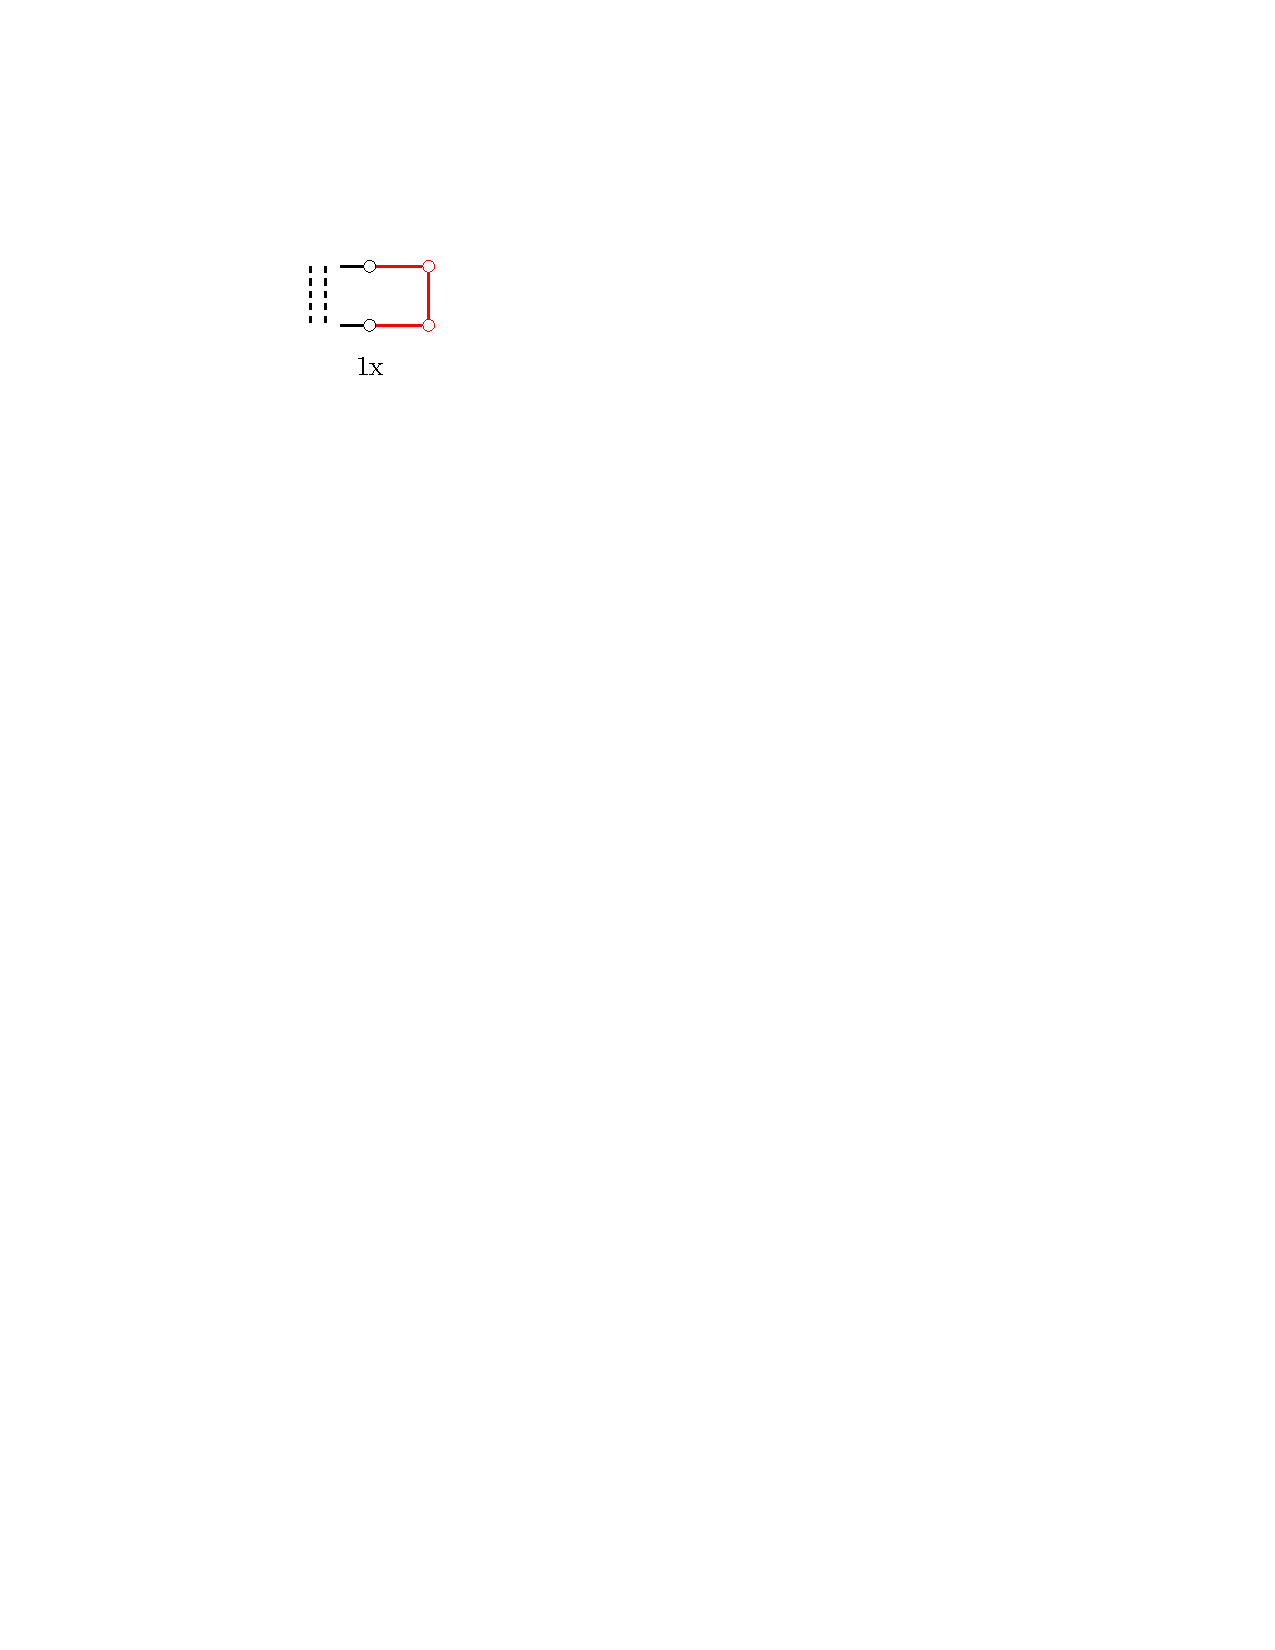
\includegraphics[trim=130 600 380 110,clip]{img/ladder_table_cell2} \\
  \hline
  \raisebox{3.7\height}{$X_B (n+1)$} & 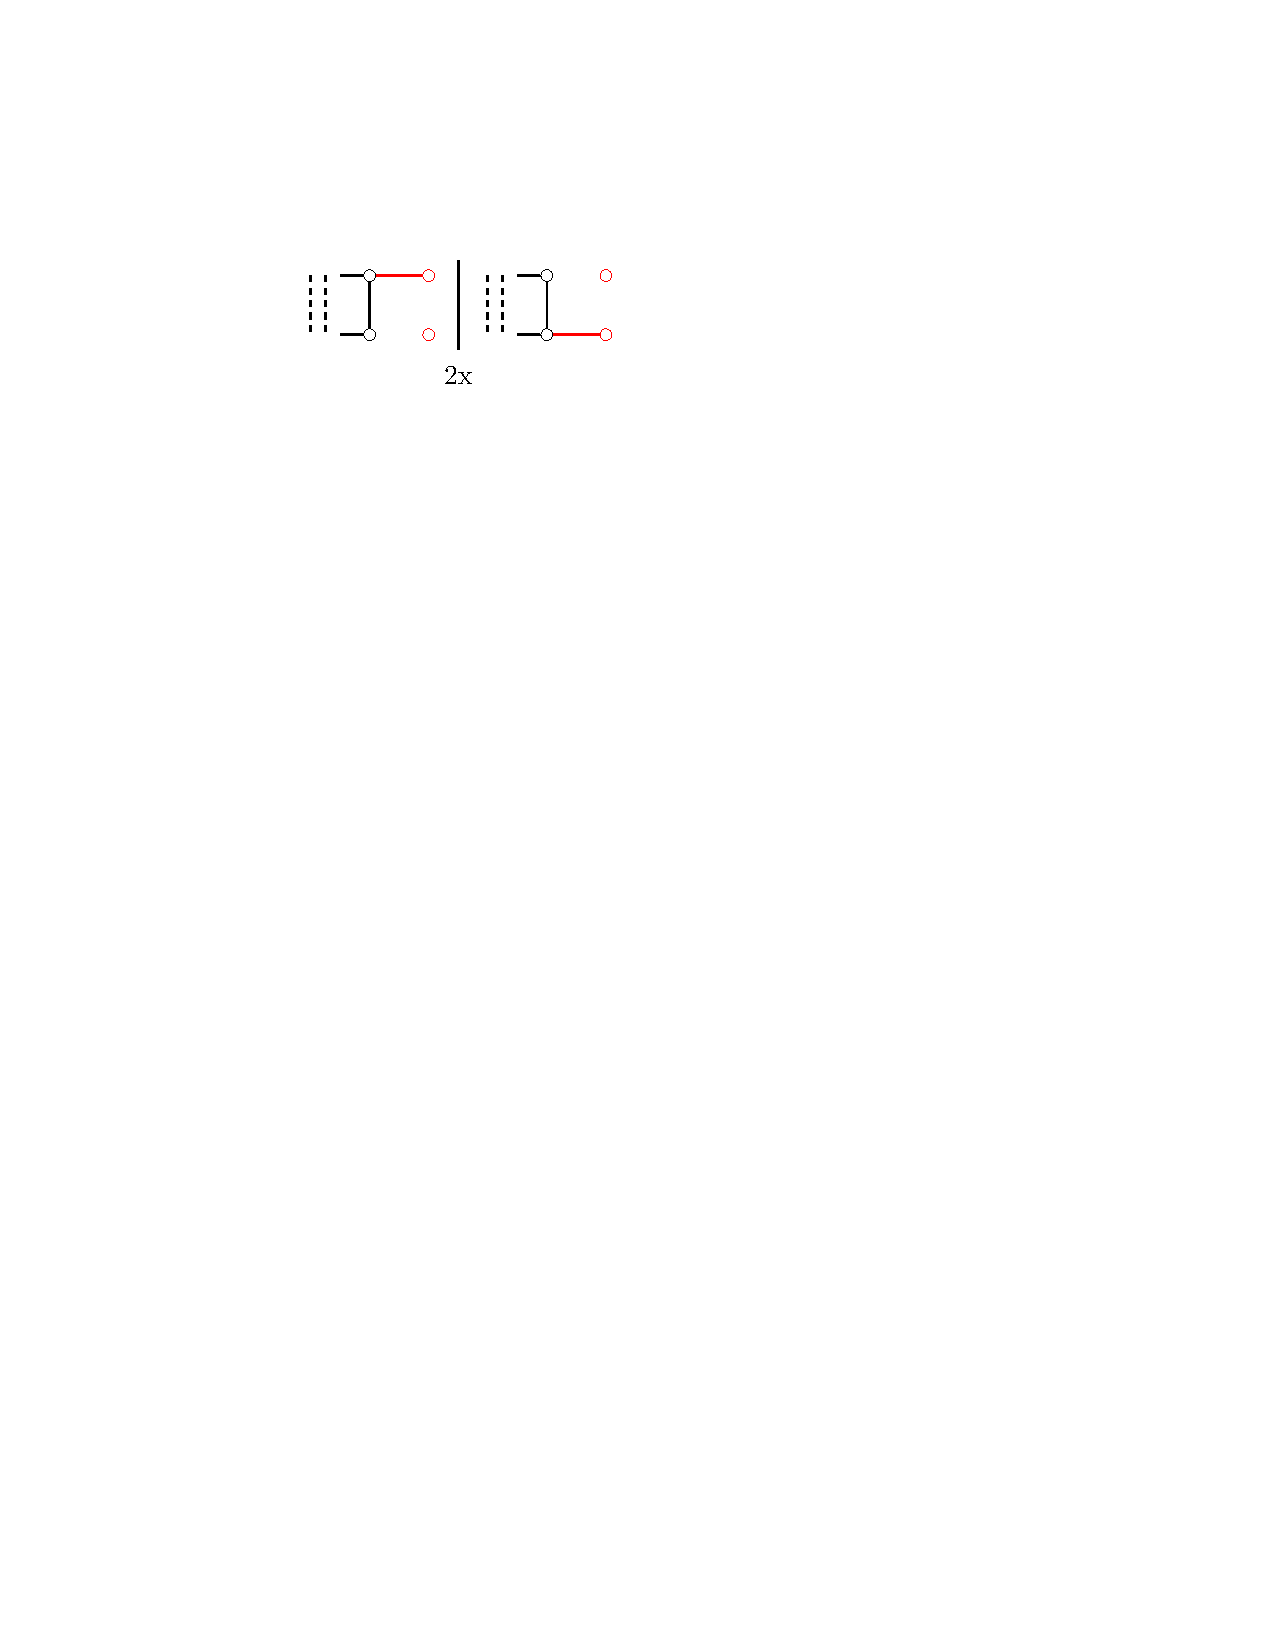
\includegraphics[trim=130 600 300 110,clip]{img/ladder_table_cell3} & 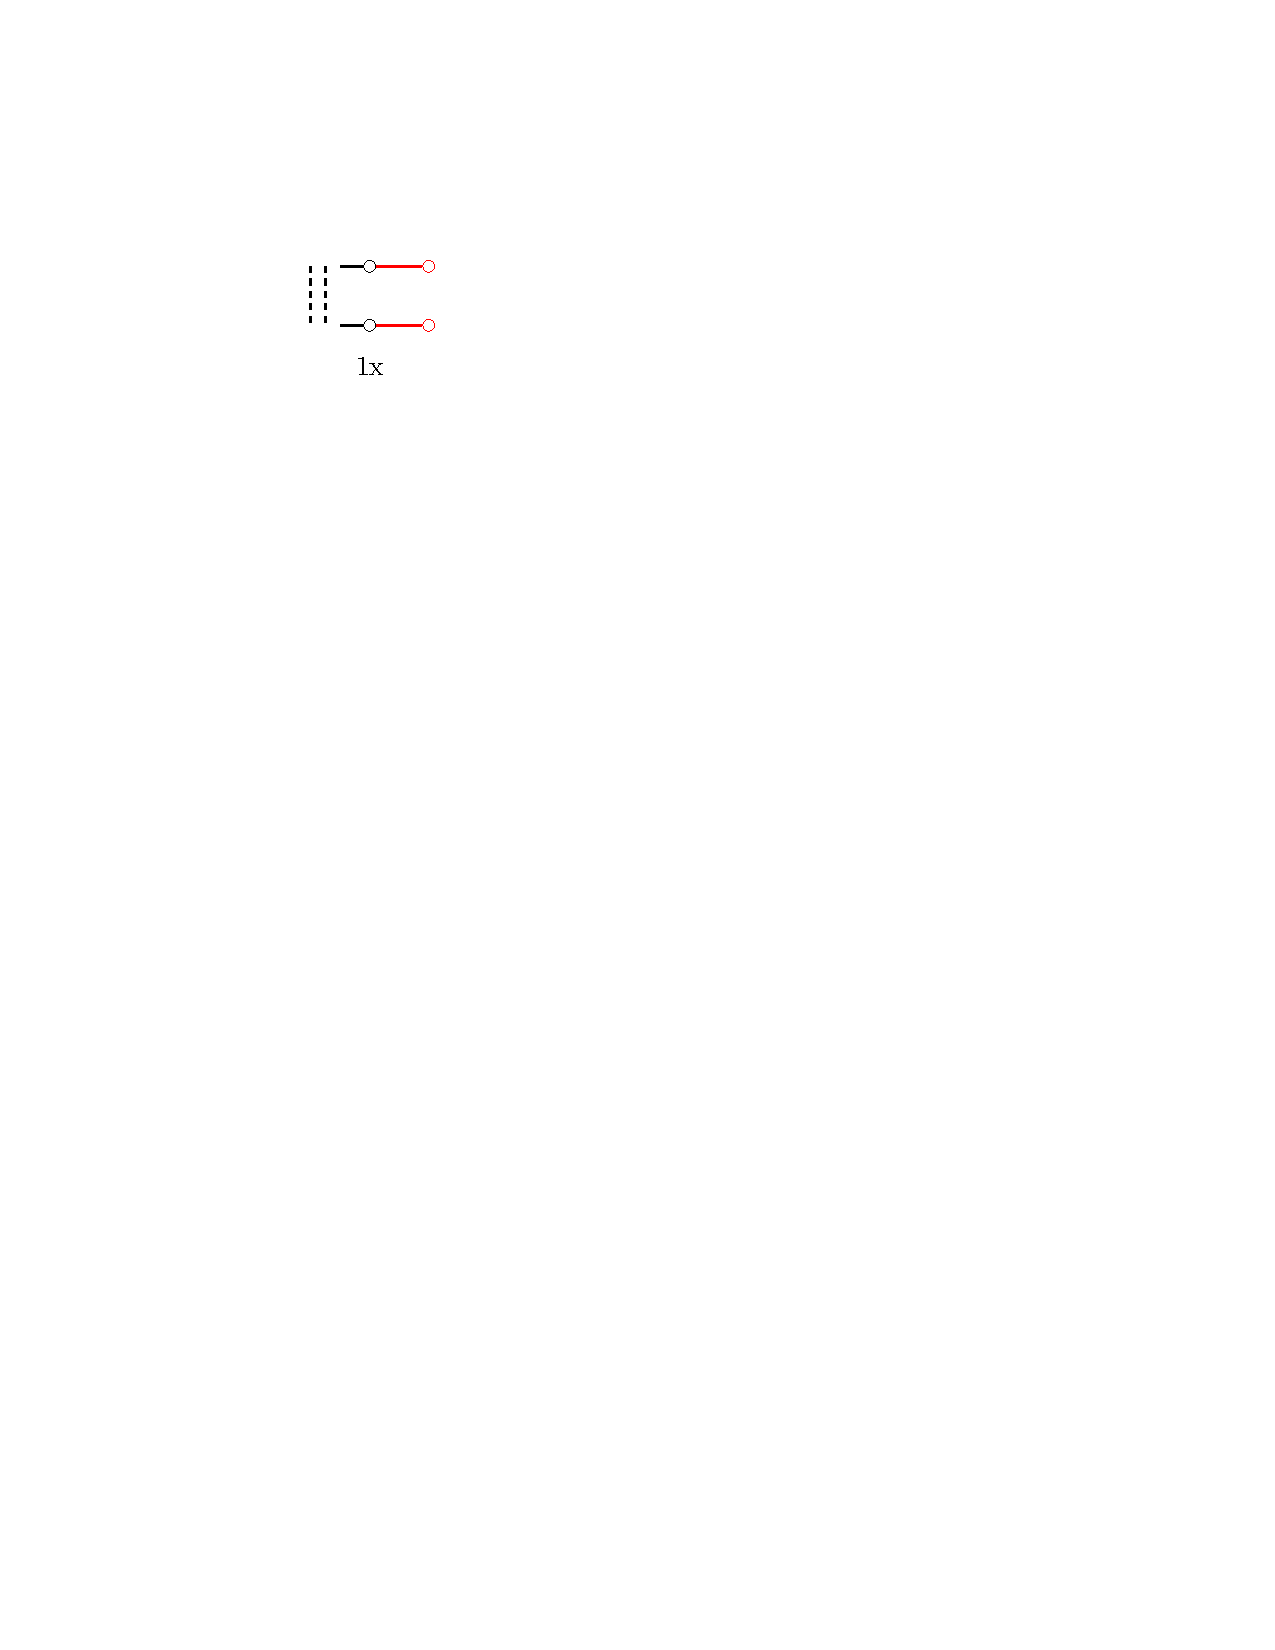
\includegraphics[trim=130 600 380 110,clip]{img/ladder_table_cell4}
\end{tabular}
\end{center}

We can translate this into a matrix.

\eq{
	X_A (1) = 1 \\
	X_B (1) = 1
}

\eq{
	\mat{X_A (n+1) \\ X_B (n+1)} = \mat{3&1 \\ 2&1} \mat{X_A (n) \\ X_B (n)} = \mat{3&1 \\ 2&1}^n \mat{1 \\ 1}
}

\eq{\text{for n: } \mat{3&1 \\ 2&1}^{n-1} \mat{1 \\ 1}}

However, we are only interested in $X_A(n)$ and want to get $X_B(n)$ out of the equation.

\eq{
	X_A(n+1) &= 3X_A(n) + X_B(n) \rightarrow X_B(n) = X_A(n+1) - 3X_A(n) \\
	X_B(n+1) &= 2X_A(n) + X_B(n) \rightarrow \underline{X_B(n)} = 2X_A(n-1) + X_B(n-1) \\
	&\rightarrow 2X_A(n-1) + X_A(n) - 3X_A(n-1) \\
	&= \underline{X_A(n) - X_A(n-1)} \\
	\\
	X_A(n+1) &= 3X_A(n) + X_A(n) - X_A(n-1) = \underline{4X_A(n) - X_A(n-1)}
}

With this recursive formula we can solve the problem easily.

\eq{
	&X_A(1) = 1 \\
	&\underline{X_A(2) = 4} \\
	&X_A(3) = 4 \cdot 4 -1 = 15 \\
	&X_A(4) = 4 \cdot 15 - 4 = 56 \\
	&\qquad \vdots
}

But, as the formula has a recursion we always need to know the last two elements. We can use linear algebra or aspects of generating functions to get rid of this recursion!

\fig{
	\eq{
		X_A(n) = \frac{1}{2 \cdot \sqrt{3}} \, (2+\sqrt{3})^n - \frac{1}{2 \cdot \sqrt{3}} \, (2-\sqrt{3})^n
	}
}{Non-recursive formula for the number of spanning trees a ladder of size $n$ contain as subgraphs}

The Asymptotics are: $\Theta((\underbrace{2+\sqrt{3}}_{3,73})^n)$

\newsection{Polya-Redfield Enumeration Theorem
aka Burnside's Lemma}

\subsection{Objects and Operations}

Set of \textbf{objects} $X$ \\
Set of \textit{n} \textbf{operations} \textit{R} = $\{R_{i},0 \leq i \leq \textit{n} - 1 \}$

R forms a group w.r.t. $\circ$ (4 axioms $\forall R_{i}, R_{j}):$  \\
Closure: $\exists R_{k} : R_{i} \circ R_{j} = R_{k}$ \\
Associativity: $(R_{i} \circ R_{j}) \circ R_{k} = R_{i} \circ (R_{j} \circ R_{k}) $ \\
$R_0$ is identity element, i.e, $R_{0} \circ R_{i} = R_{i} \circ R_{0} = R_{i}$ \\
Inverse element: $\exists R_{k} : R_{k} \circ R_{i} = R_{i} \circ R_{k} = R_{0}$ 

\textbf{Objects} might be strings, colored grids, colored cubes, ... \\
\textbf{Operations} might be rotations, reflections, ... \\
For objects, $R_{0}$ is the identity (neutral) function.

\subsection{Orbits}
An orbit is the set of all objects from $X$ which can be
transformed into each other by an operation from $R$
(equivalence class).
The length of an orbit is the number of elements it
contains.
\begin{center}
\textbf{Main Question: How many Orbits exist?}
\end{center}

\subsection{Stabilizers}
For an object $x \in X$ the operation $R_{i} \in R$ is a \textbf{stabilizer} \\
if and only if $R_{i}(x) = x$.

$m_{x}$ ... number of stabilizers for $x$ \\
$r_{i}$ ... invariance number, i.e., number of objects for which
$R_{i}$ is a stabilizer.

We have $\sum \limits_{i = 0}^{n - 1} r_{i} = \sum \limits_{x \in X} m_{x}$
by double counting (each pair operation/object which gives
an invariance is counted once on each side; left side counts
by operation, right side counts by objects).

\subsection{Counting Orbits}
Deriving a first relation { simplified version (not valid in full
generality):\\
$ \sum \limits_{x \in orbit} m_{x} = n $

\noindent
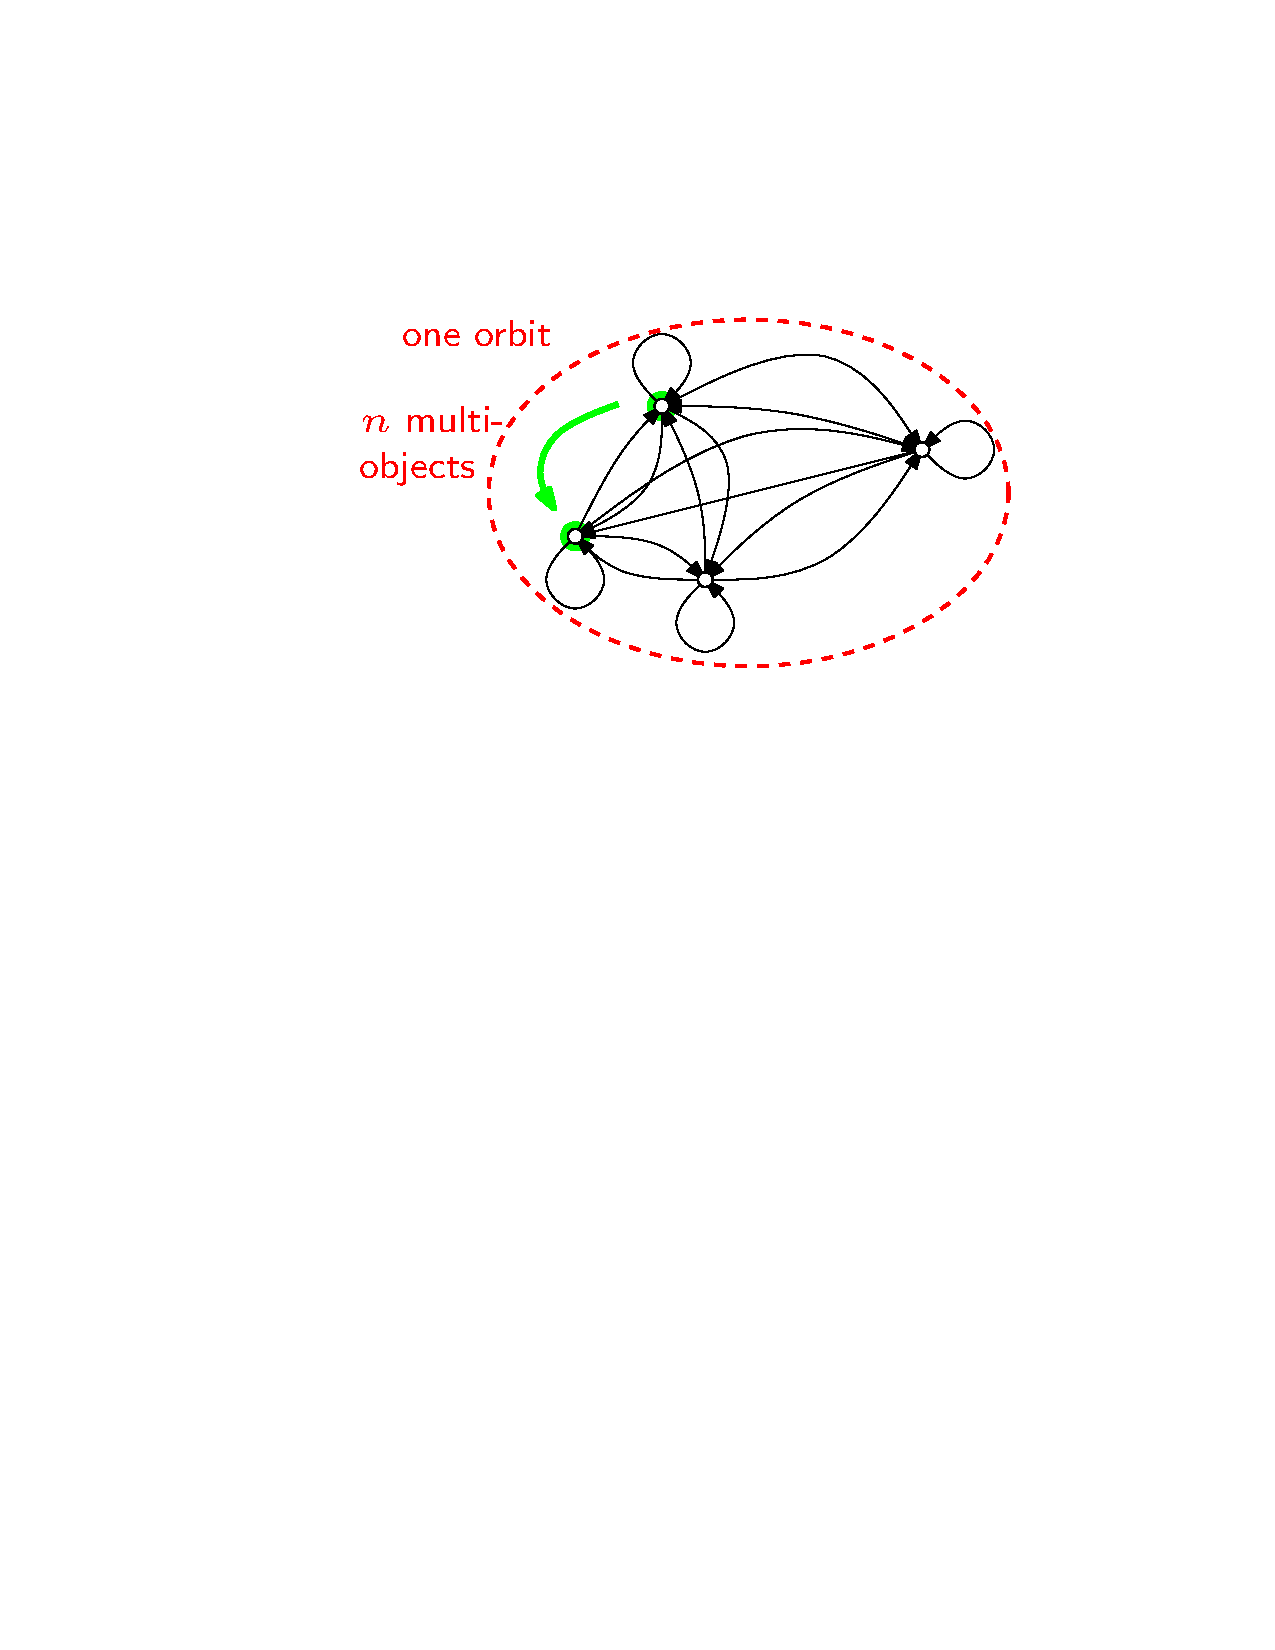
\includegraphics[scale=0.6, trim=170 460 125 150, clip]{img/orbit_left}
\begin{minipage}[b]{0.33\textwidth}
\centering
Two times the same
object: unify the vertices! \\
For removed copy: remove
outgoing edges, reroute
incoming edges. \\
We get one new stabilizer! $\rule{1cm}{0mm}$
\end{minipage}
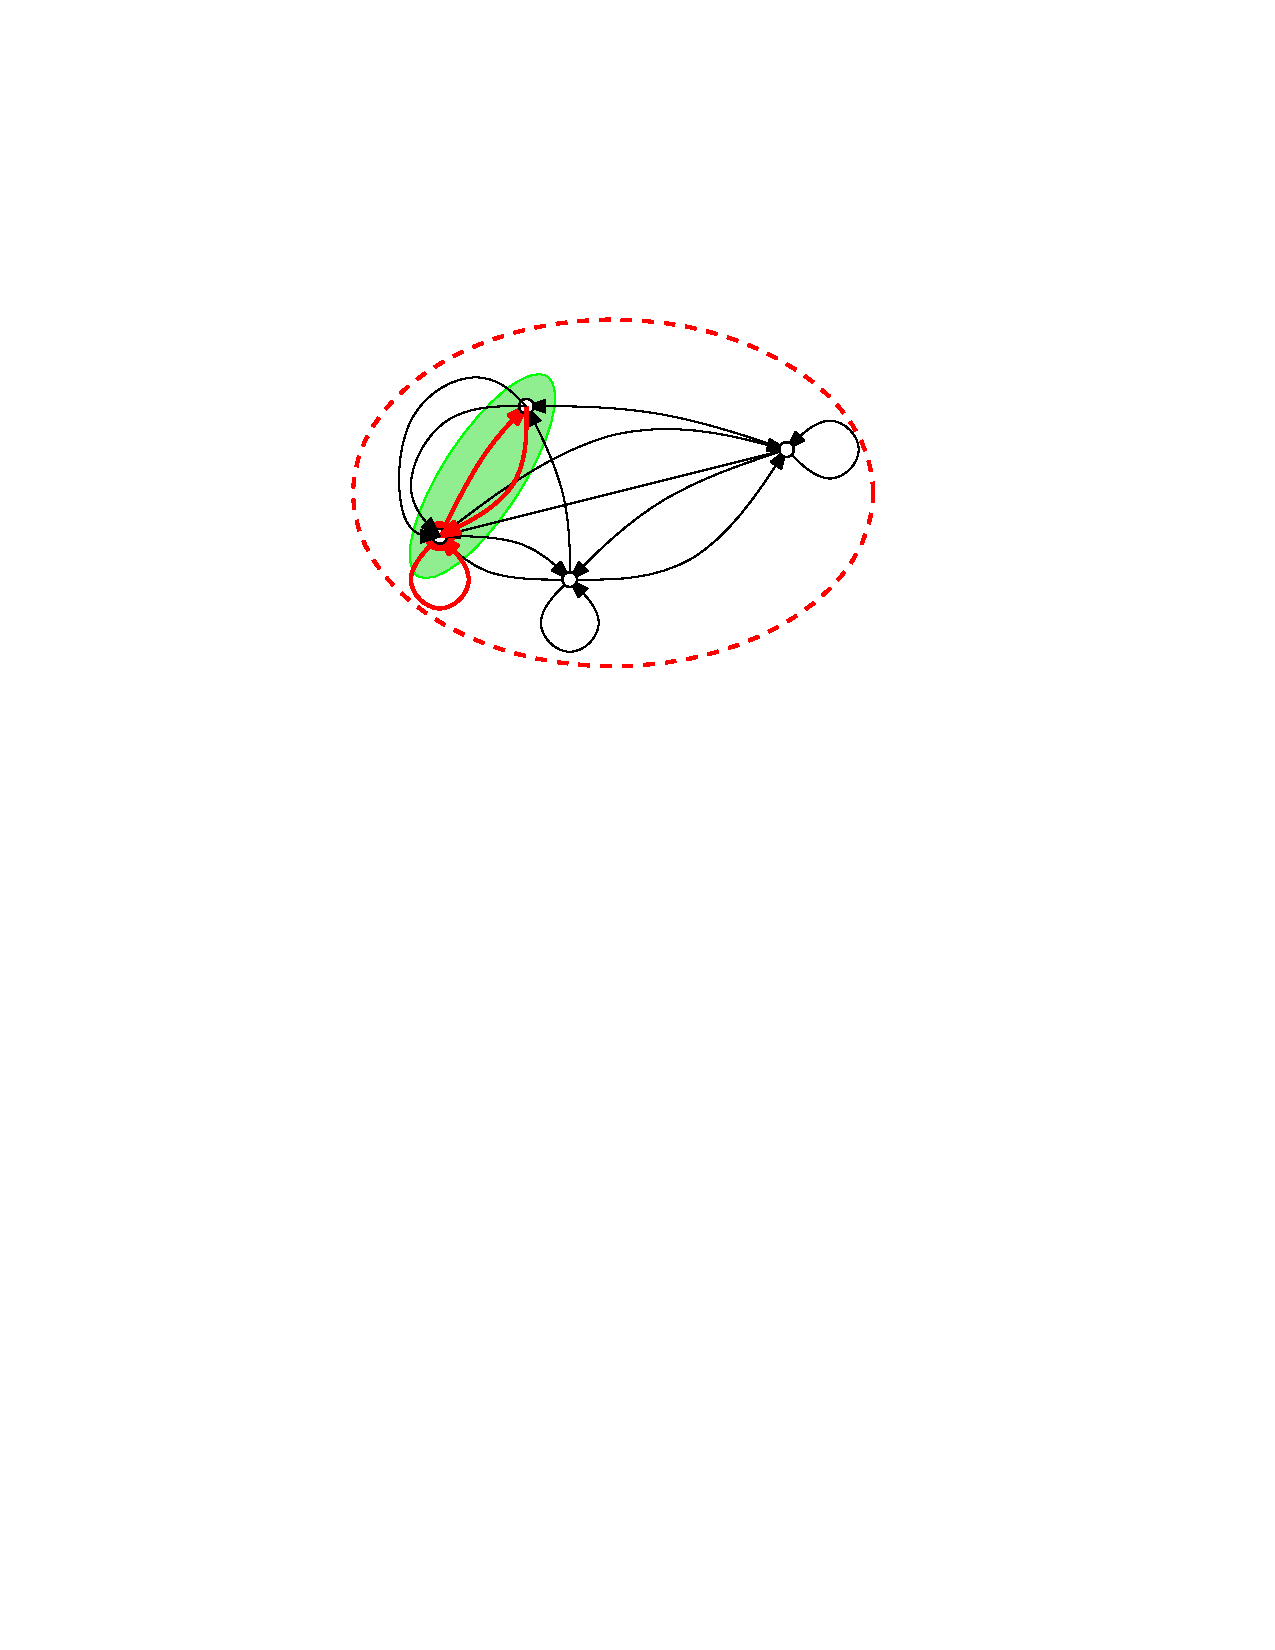
\includegraphics[scale=0.6, trim=165 460 125 150, clip]{img/orbit_right}

This leads to the formula: \\
number of orbits = $\frac{\sum \limits_{x \in X} m_{x}}{n}$ \\
With the previous observation $\sum \limits_{i = 0}^{n - 1} r_{i} = \sum \limits_{x \in X} m_{x}$
we therefore get
\begin{center}
\colorbox{yellow}{number or orbits = $\frac{\sum \limits_{i = 0}^{n - 1} r_{i}}{n}$}
\end{center}
We will use this equation, as usually $n << |X|$ and thus,
all invariance numbers $r_{i}$ are easier to obtain than all
numbers $m_{x}$ of stabilizers.

\subsection{Examples}
\subsubsection{Strings (1)}
Consider strings of length 4 with characters $\{A,B\}$\\
Operation: cyclic shift by $i$ positions, $0 \leq i \leq 3$. How many
different strings exist?

Algorithm:
\begin{center}
\begin{enumerate}
\item Identify $R_{0}$ to $R_{n-1}$ \\
\item Compute all invariance numbers $ r_{i},0 \leq i \leq n - 1$ \\
\item Compute the number of orbits $\frac{\sum \limits_{i = 0}^{n - 1} r_{i}}{n}$
\end{enumerate}
\end{center}

We have 4 shift operations, therefore we have the operations $R_{0}$ to $R_{3}$ \\
$R_0$ - 0 Shifts: $r_{0} = 2^{4} = 16$ : 2 characters for 4 positions \\
$R_1$ - 1 Shift: $r_{1} = 2$ : \st{A}{A}{A}{A} or \st{B}{B}{B}{B} \\
$R_2$ - 2 Shifts: $r_{2} = 4$ : \st{A}{A}{A}{A} , \st{B}{B}{B}{B}, \st{A}{B}{A}{B} or \st{B}{A}{B}{A} \\
$R_3$ - 3 Shifts: $r_{3} = 2$ : The same as for $r_{1}$

\raisebox{2.5\height}{$r_1$ follows the following pattern:} 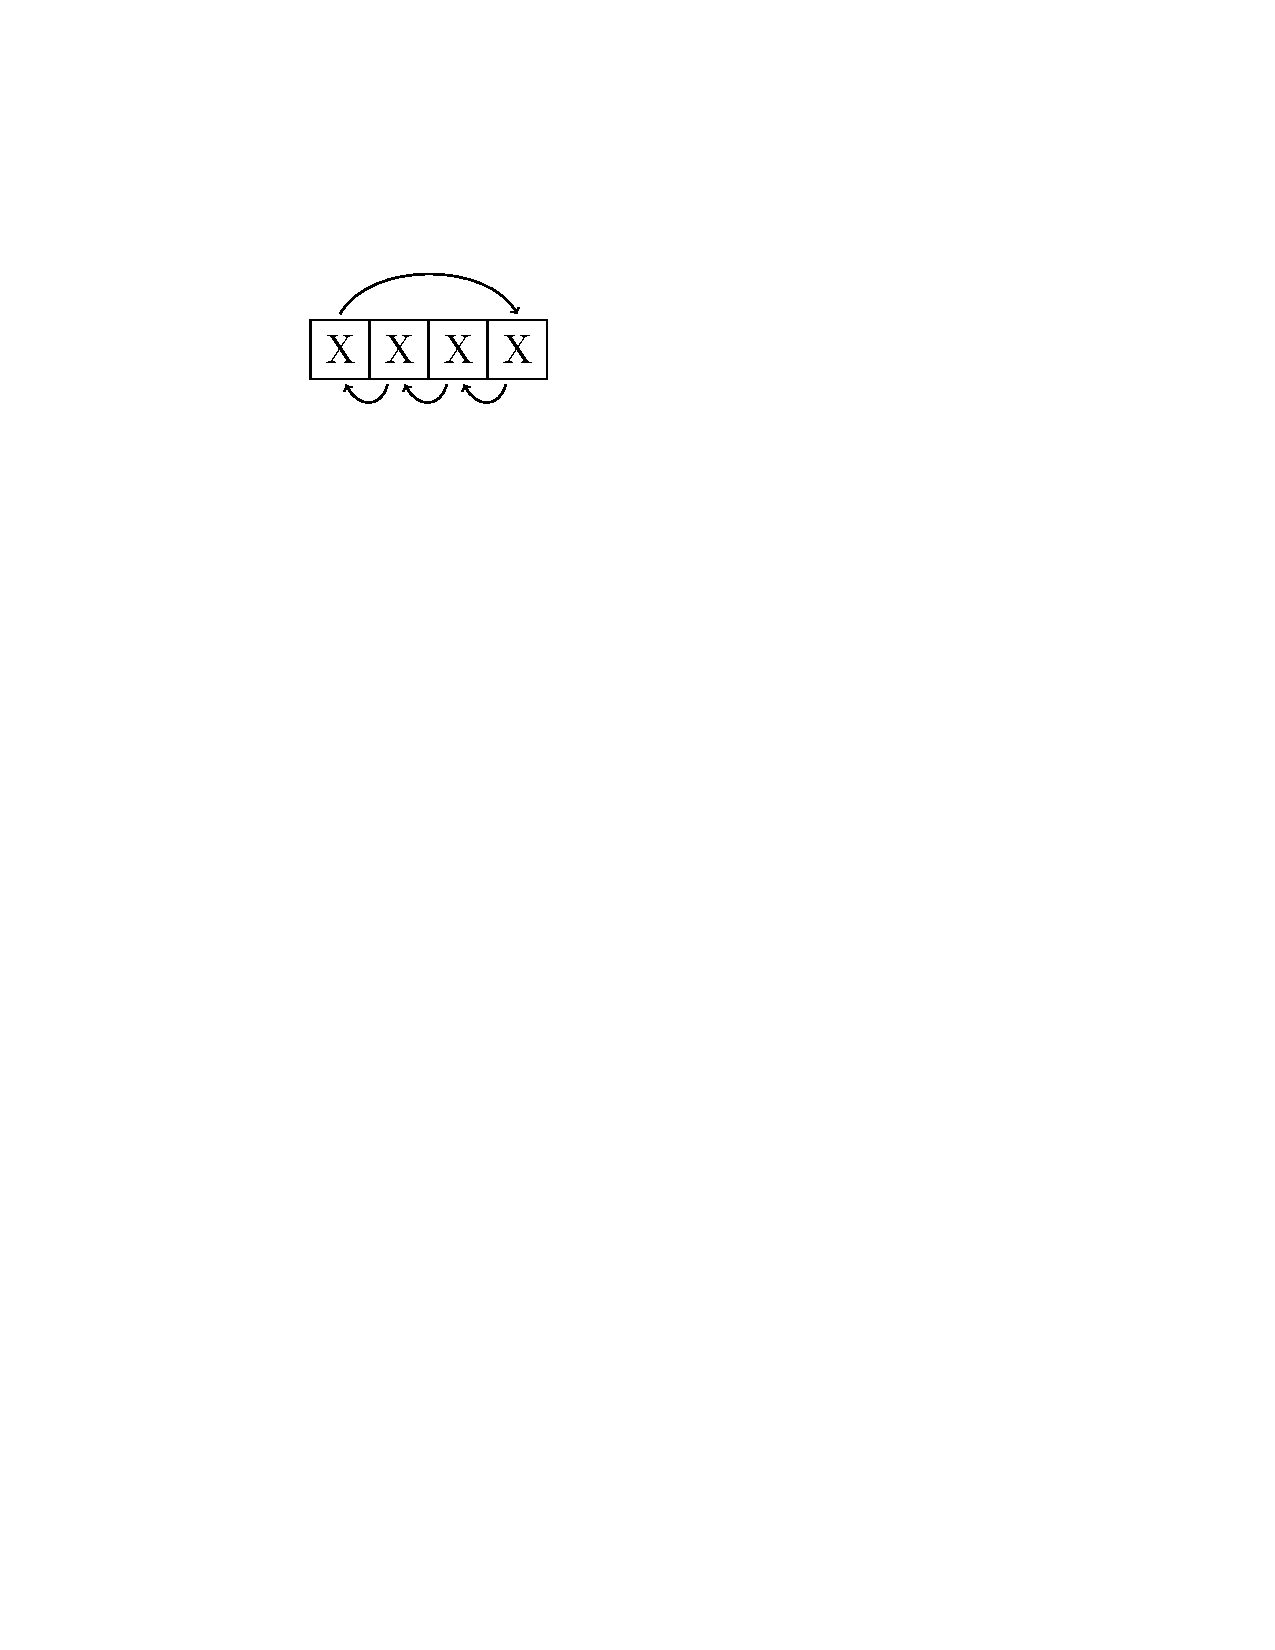
\includegraphics[scale=0.6,trim=140 585 345 130, clip]{img/group_XXXX} \raisebox{2.5\height}{and $r_2$:} 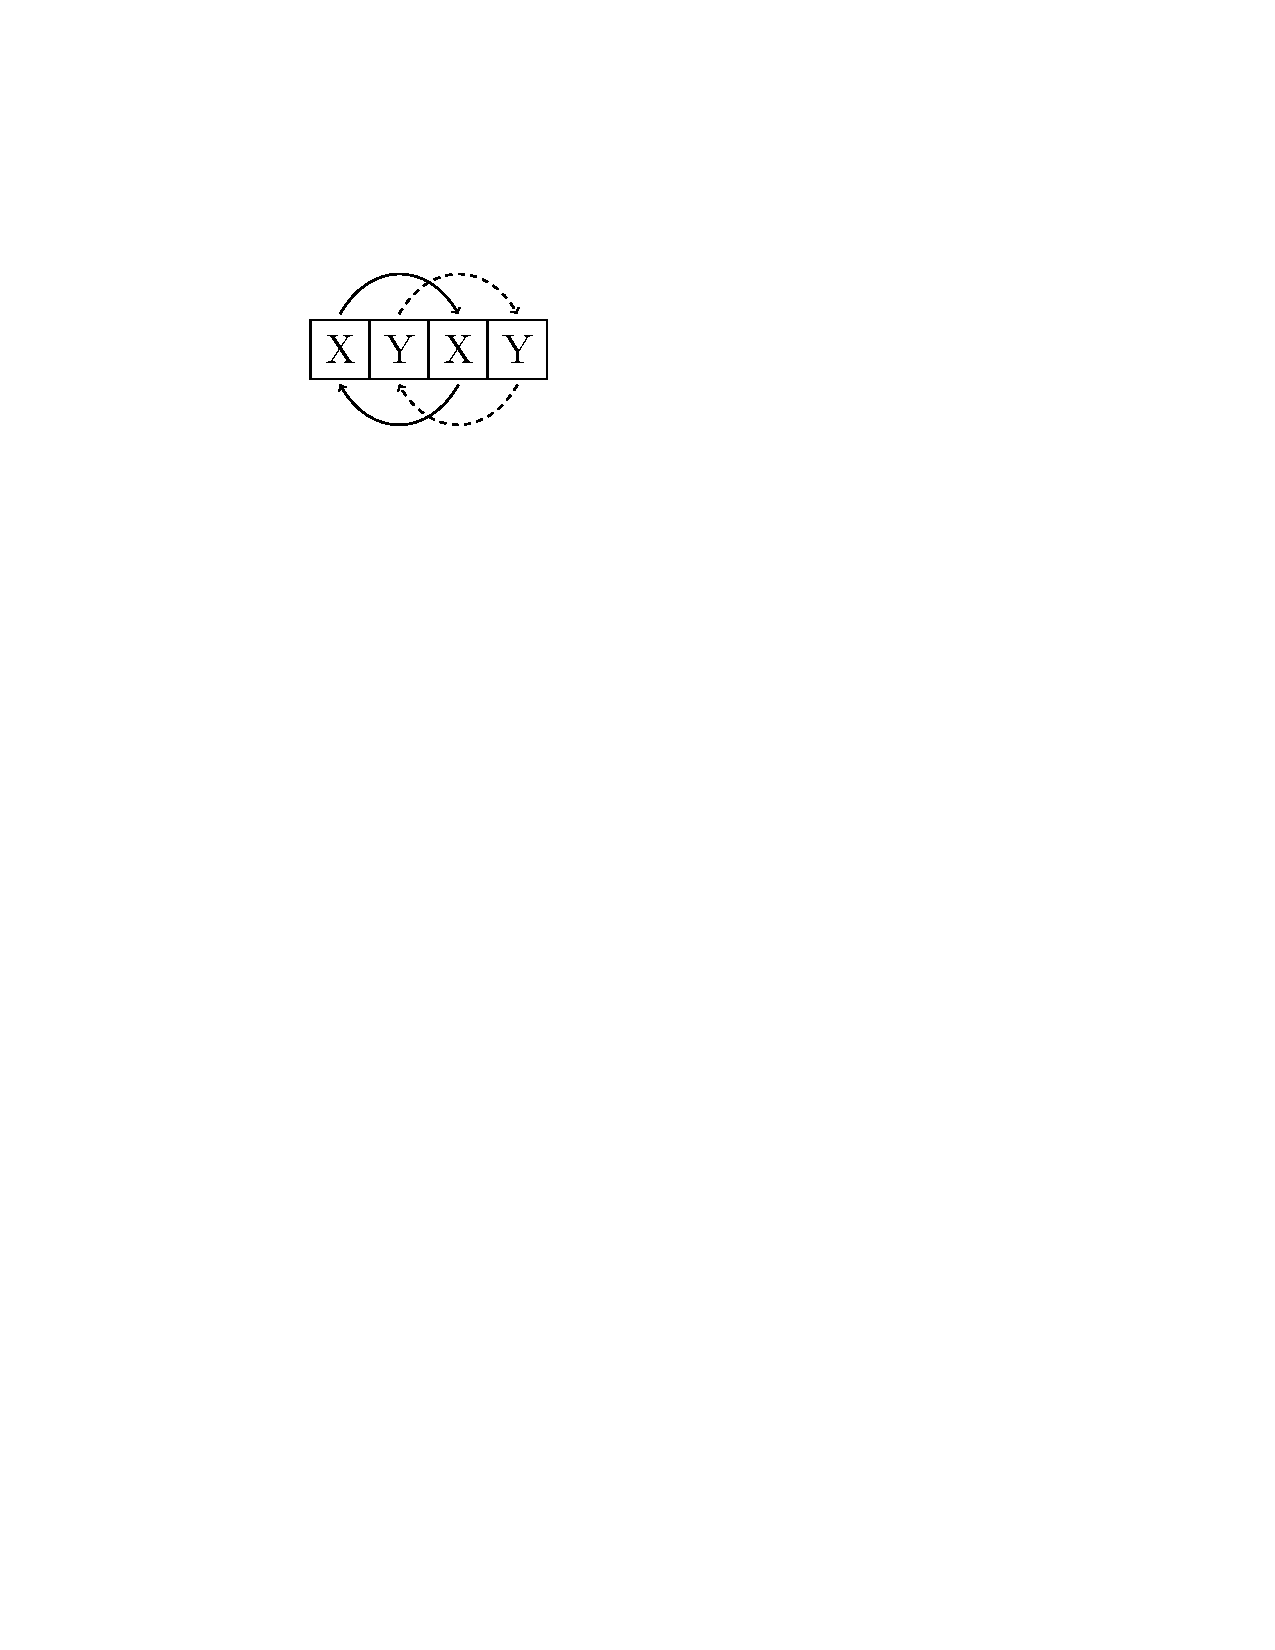
\includegraphics[scale=0.6,trim=140 585 345 130, clip]{img/group_XYXY} \\
X and Y are used to symbolize the boundaries between different groups. \\

number of orbits = $ \frac{16+2+4+2}{4}$ = $ \frac{24}{4} $ = \textbf{6}

But how? - write down the 16 possibilities ($R_{0}$) and group them into their orbits.
That means that groups are formed by strings that are basically the same but shifted. \\

\colorbox{yellow}{AAAA} ... Yellow is Orbit 1\\
\colorbox{red}{AAAB} ... Red is Orbit 2\\
\colorbox{red}{AABA} \\
\colorbox{red}{ABAA} \\
\colorbox{red}{BAAA} \\
\colorbox{green}{AABB} ... Green is Orbit 3  \\
\colorbox{orange}{ABAB} ... Orange is Orbit 4\\
\colorbox{green}{ABBA} \\
\colorbox{green}{BAAB} \\
\colorbox{orange}{BABA} \\
\colorbox{green}{BBAA} \\
\colorbox{gray}{ABBB} ... Gray is Orbit 5\\
\colorbox{gray}{BABB} \\
\colorbox{gray}{BBAB} \\
\colorbox{gray}{BBAB} \\
\colorbox{gray}{BBBA} \\
\colorbox{pink}{BBBB} ... Pink is Orbit 6 \\

There we can clearly see the 6 different orbits.

\subsubsection{Strings (2)}
This is the same example as the previous one, but with the character-set $\{A,B,C\}$ \\
$r_{0} = 3^{4} = 81$, which determines all possible ways the characters can be set \\
$r_{1} = r_{3} = 3$, which determines the 3 ways you can set the characters when shifting by 1 or 3
characters and the meaning stays the same.

Those are: \st{A}{A}{A}{A}, \st{B}{B}{B}{B} and \st{C}{C}{C}{C} \\
$r_{2} = 9$. The basic idea behind this is that you can shift 2 times when a string consist of only 1 character
like \st{A}{A}{A}{A} or has the form \st{X}{Y}{X}{Y} or \st{Y}{X}{Y}{X}. With 3 available characters we get those 9 ways.\\

This gives us the number of orbits: $\frac{96}{4} = 24$

\subsubsection{Strings (3)}
This is the same example as Example String (2), but you have to use every character atleast once.
$r_{0} = 36$\\
$r_{1} = 0$\\
$r_{2} = 0$\\
$r_{3} = 0$\\

Why is it 36?\\
We know when every character has to be there 1 time, one character has to be there 2 times.\\
So we have 3 characters that can be chosen twice.\\
Then we have 2 characters left from the 4 character long string. \\
At the end we have 2 possibly ways to fill the 2 characters which are left. For example:
\st{B}{A}{C}{A} and \st{C}{A}{B}{A} \\

Therefore we get $3 \times\begin{pmatrix}4\\2\end{pmatrix}\times 2$ \\
$\begin{pmatrix}4\\2\end{pmatrix} = 6$ so we have $3 \times 6 \times 2 = 36$\\

This gives us the number of orbits: $\frac{36+0+0+0}{4} = 4$

\subsubsection{Grids (4)}

Consider a 2x2 grid as shown below. Color the unit squares with up to 2 different colors. How many {\bf different} colorings exist, if we allow (a) rotation (b) rotation and reflection?

\imgnc{block_2x2}{trim=140 610 400 120, clip}

\img{block_2x2_rot}{scale=1.1,trim=140 350 335 125, clip}{$R_0$ to $R_3$, rotation by 0, 90, 180 or 270 degrees.}

$r_0 = 2^4 = 16$ : 2 colors on 4 unit-squares. \\
$r_1 = 2$ : all red or all blue. \\
$r_2 = 2^2 = 4$ : $r_1$ + diagonals \\
$r_3 \sim r_1 = 2$

\img{block_2x2_groups_rot}{trim=140 530 245 130, clip}{Grouping for $r_1$ and $r_2$ in regards to rotation.}

We still need to take a look at $R_4$ to $R_7$, our operations concerning reflection. We allow horizontal and vertical reflection as well as reflection on either diagonal axis.

\img{block_2x2_groups_ref}{trim=140 440 235 120, clip}{Grouping for $r_4$ to $r_7$ in regards to reflection.}

$r_4 = 2^{2 \text{ groups}} = 4$ \\
$r_5 = 2^{2 \text{ groups}} = 4$ \\
$r_6 = 2^{3 \text{ groups}} = 8$ \\
$r_7 = 2^{3 \text{ groups}} = 8$

\eq{
	\text{(a) }& \frac{16+2+4+2}{4} = \frac{24}{4} = 6 \\
	\text{(b) }& \frac{16+2+4+2+4+4+8+8}{8} = \frac{48}{8} = 6
}

\end{document}
